\section{Scenario A: Push Notifications}
As previously mentioned, the goal of push notifications is to recommend relevant and
novel tweets based on the user’s interest profile in real-time.
At a high level, push notifications should be relevant (on topic),
timely (provide updates as soon after the actual event occurrence as possible),
and novel (users should not be pushed multiple notifications that say the same thing).
In this section, we mainly describe the architecture of our proposed system, which is shown in \ref{fig:a}.

\begin{figure}[htbp]
\centering {
	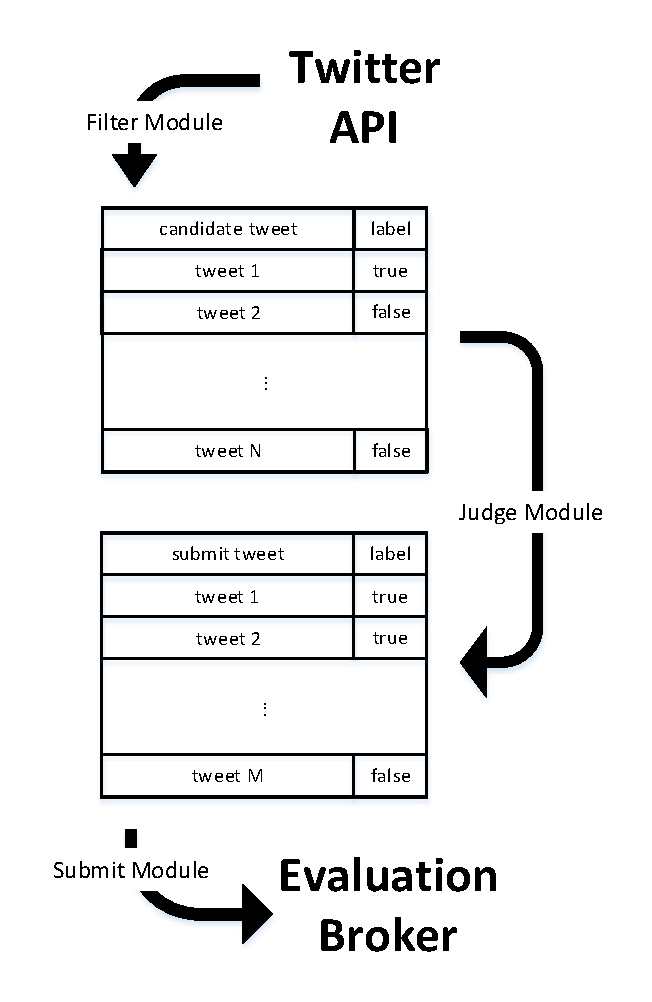
\epsfig{file=figures/a.pdf, width=0.35\textwidth}
}
\caption{The System Architecture of the Push Notifications Scenario.}
\label{fig:a}
\end{figure}

From the figure, we can observe that our system mainly contains three processes and two storage tables:

\begin{itemize}
\item \textbf{Filter Module:} 
In order to accelerate the speed of identifying possible relevant tweets for each profile,
We first build a interest vocabulary based on all words in the given users' interest profiles.
Then, the Twitter sample stream is obtained via the Twitter API.
For each crawled tweet, we check whether it contains any words in our interest vocabulary.
If contains, we insert it into our candidate tweets storage table. If not, filter it.
In this way, we simply ignore tweets that do not contain any keywords for each profile.

\item \textbf{Judge Module:}
This process keeps ``listening'' to the candidate tweets storage table.
In every $T1$, it selects at most $K1$ untreated candidate tweets and compare them with the given users' interest profiles.
For each (tweet, profile) pair, we first calculate the relevant score between them by the text similarity function $f$.
If the relevant score is bigger than $\alpha$, we then compute similarity scores between this tweet and all pushed tweets of this profile
via the text similarity function $f$, the biggest one will be chosen as the novel score.
If the novel score is smaller than $\beta$, we will insert it into the submission tweets storage table.
In the last, these selected tweets will be set to treated or removed from the storage table.

\item \textbf{Submit Module:}
This process keeps ``listening'' to the submission tweets storage table.
In every $T2$, it selects at most $K2$ untreated submission tweets and try to submit them to the evalation broker one by one.
If return code is $204$ for one tweet, which means the remote server accepted it successfully,
we will set the submitted tweet treated or remove it from the storage table.
Otherwise, the tweet is going to handle in the next round until accepted.
\end{itemize}

\subsection{Similarity Algorithm}
We utilize the negative KL-divergence language model for $f$ and $g$ to measure the relevance between
query language model $\widehat{\theta}_Q$ and tweet language model $\widehat{\theta}_D$
with the help of collection lanuage model $\widehat{\theta}_C$.
The smoothing methods we use for language model are:

(a) Jelinek-Mercer Smoothing
\begin{equation}
\begin{aligned}
JM(Q,&D,C) = \sum_{w \in Q} P(w|\widehat{\theta}_Q) \cdot \\
&log \left( (1-\lambda) * P(w|\widehat{\theta}_D) + \lambda * P(w|\widehat{\theta}_C) \right)
\end{aligned}
\end{equation}

(b) Dirichlet Smoothing
\begin{equation}
DIR(Q,D,C) = JM(Q,D,C), \lambda = \frac{\mu}{|D| + \mu}
\end{equation}

\subsection{Parameter Selection}
The $T1$ and $T2$ are both set to $10$ seconds.
$K1$ is set to $1000$ while $K2$ is set to $10$ due to their different scale.
Those parameters are set empirically and mainly depend on your computer performance.
$\alpha$ and $\beta$ are tuned via grid search on TREC 2015 dataset,
which is showed in Table \ref{tab:paraA}.

\begin{table}[htbp]
\centering
\caption{Parameters of the Push Notifications Scenario.}
\label{tab:paraA}
\begin{tabular}{lccc}
\hline
Run ID&f&$\alpha$&$\beta$\\
\hline
PKUICSTRunA1&JM($\lambda=0.2$)&0.79&0.72\\
PKUICSTRunA2&JM($\lambda=0.5$)&0.85&0.74\\
PKUICSTRunA3&DIR($\mu=100$)&0.75&0.68\\
\hline
\end{tabular}
\end{table}


